\section{Architektur}

\subsection{Allgemein}

\noindent Die Basis eines \acp{GAN} bilden wie bereits erwähnt zwei Modelle, der Generator und der Diskriminator. Diese beiden Modelle agieren als Gegenspieler und trainieren einander, um zu einem besseren Gesamtresultat zu führen. Somit gehören beide Komponenten stets zueinander und sind jeweils beide für die korrekte Funktion der Architektur unverzichtbar. Die Daten, mit welchen die Modelle arbeiten, können in Form von verschiedenen Formaten definiert sein, wie Bildern, Texten oder sogar Musik, in den nachfolgenden Kapiteln wird allerdings ausschließlich der visuelle Aspekt von \acs{GAN} betrachtet. Dabei unterscheiden sich die Arbeitsweisen der beiden Modelle grundlegend: \\

\noindent \textbf{Generator:} Der Generator erzeugt neue Daten, die echten Daten möglichst ähnlich sehen sollen. Es ist das Modell der beiden, welches nach dem Abschließen des Trainings für die tatsächliche Generation von neuen Daten verwendet wird. Der Generator wird mit zufälligem Rauschen als Eingabe gestartet, welches als Latent Space bezeichnet wird. Dieses Rauschen in Form eines Vektors wird als Eingabe in den Generator eingespeist, welcher durch das Feedback des Diskriminators im Laufe der Zeit lernt, Daten zu erzeugen, die von einem echten Datensatz nicht zu unterscheiden sind. Dieser Prozess wird auch als \textit{Backpropagation} bezeichnet und erlaubt das unüberwachte Lernen der Netze. \\

\noindent \textbf{Diskriminator:} Der Diskriminator hat die Aufgabe, zwischen echten Daten und den vom Generator erzeugten Daten zu unterscheiden. Er wird mit einer Mischung aus echten und generierten Daten trainiert und wird nach Abschluss des Trainings für die eigentliche Generation von Bildern nicht mehr benötigt, ist jedoch dennoch für das Training des \acp{GAN} unverzichtbar. Der Diskriminator lernt, die beiden Arten von Daten auseinanderzuhalten, indem er die Wahrscheinlichkeit berechnet, mit welcher das aktuelle Objekt künstlich erzeugt wird, woraufhin eine binäre Klassifikation durchgeführt wird, welche eine binäre Entscheidung festlegt und die Korrektheit der Entscheidung auswertet. Dies ist möglich, da der Diskriminator im Gegensatz zum Generator Zugriff auf die Realdaten hat und geschieht ebenfalls durch Backpropagation. \\

\noindent Der Prozess des Trainings wird in einem nachfolgenden Kapitel noch näher behandelt. 

\newpage

\begin{figure}[h]
    \centering
    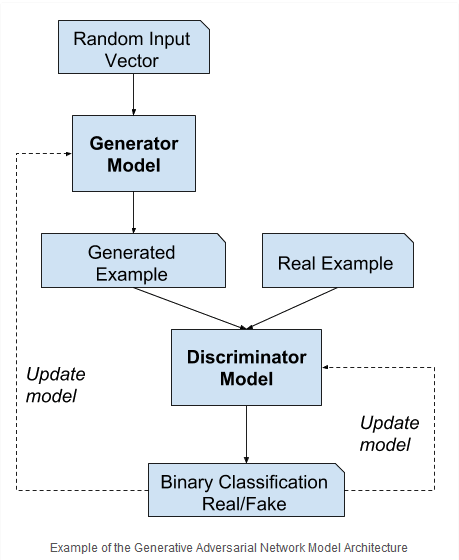
\includegraphics[width=0.6\textwidth]{GAN_Model}
    \caption{Funktionsprinzip eines \ac{GAN}}
    \label{Abb:basic}
    \end{figure}

    \noindent Die Abbildung zeigt die grundlegende Architektur eines \ac{GAN}, wie es auch schon in den Grundlagen zuvor erklärt wurde. Der Generator erhält als Eingabe einen zufälligen Vektor, der als Latent Space bezeichnet wird. Dieser Vektor wird als Eingabe in den Generator eingespeist und durchläuft eine Reihe von Schichten, die jeweils eine Reihe von Neuronen enthalten. Die letzte Schicht des Generators, die Ausgabeschicht, gibt einen Vektor aus, der die generierten Daten enthält. Der Diskriminator erhält schließlich als Eingabe entweder diesen oder einen aus echten Daten stammenden Vektor als Eingangswert. Dieser Vektor durchläuft anschließend einen ähnlichen Prozess, wie der Latent Space in Form des Diskriminators. Die letzte Schicht des Diskriminators gibt schließlich einen Vektor aus, der die Wahrscheinlichkeit angibt, ob die Eingabe aus echten oder generierten Daten besteht. Diese Wahrscheinlichkeit bietet in Form der \textit{Backpropagation} die Grundlage für das Training beider Modelle, allerdings auf zwei unterschiedliche Arten und Weisen. Sollte der Diskriminator nämlich falsch liegen und beispielsweise ein künstlich generiertes Bild als real anerkennen, so gilt dies für den Generator als Erfolg, für den Diskriminator allerdings als Fehlschlag. Dieses Verhältnis der beiden Modelle kann durch eine Funktion, die sogenannte \textit{Minimax-Verlustfunktion} \ref{eqn:Verlustfunktion} beschrieben werden.\\

    \begin{equation}
        \label{eqn:Verlustfunktion}
        L_{GAN}=\frac{1}{N_1}\sum_{i=1}^{N_1} \ln{D (\textbf{x}_i)} + \frac{1}{N_2}\sum_{j=1}^{N_2} \ln{(1-D (G (\textbf{z}_j)))}
        \end{equation}

    \noindent Der Diskriminator versucht dabei den oberen Term zu maximieren, indem korrekt zwischen echten und generierten Daten unterschieden wird. Der Generator hat allerdings die Fähigkeit den zwei Term zu beeinflussen, welchen er zu minimieren versucht. Diese Balance zwischen den beiden Modellen und ihren gegenseitigen Einflüssen, wird durch diesen Term gezeigt, welcher seinen Namen \textit{Minimax} exakt aufgrund dieser Eigenschaft besitzt. \\

\subsection{Variationen}

\noindent Die Grundlagen der Funktionsweise eines \acp{GAN} sind nun bekannt, wobei einige Parameter, wie die Art der eingesetzten Modelle generell gehalten werden und von der verwendeten GAN-Art abhängen. Außerhalb dessen existieren viele weitere Variationen der Architektur, die sich in der Regel auf bestimmte Anwendungsfälle spezialisieren. Die Grundlagen der Funktionsweise bleiben allerdings bei allen Variationen gleich. \\

\begin{description}
    \item[Conditional GAN] Ein bekanntes Beispiel für eine Erweiterung der \ac{GAN}-Architektur ist die Verwendung von Datenlabels. Diese Datenlabel werden in der Regel von Menschenhand erstellt und geben an, ob ein Bild beispielsweise eine Katze oder einen Hund zeigt. Diese Datenlabel können nun in den Trainingsprozess mit einbezogen werden, indem der Diskriminator nicht nur zwischen echten und generierten Daten unterscheidet, sondern auch zwischen den verschiedenen Klassen, die durch die Datenlabel definiert werden. Dieser Prozess wird als \textit{Conditional GAN} bezeichnet und besitzt in der Praxis meist einen größeren Nutzen für die Bildgeneration als ein einfaches \ac{GAN}. Dessen Generator wird nämlich lediglich durch den randomisierten Eingang gesteuert, welcher es nicht zulässt Einfluss auf die Ausgabe zu nehmen. Die Ausgabe ist also zufällig. Bei einer Conditional GAN hingegen, kann dem Generator zusätzlich bestimmte Eingangsbedingungen mitgegeben werden, die beispielsweise den Stil oder das Motiv des resultierenden Bildes beeinflussen können.

    \newpage

    \item[Deep Convolutional GAN] Eine weitere Möglichkeit der Verbesserung der Architektur sind die sogenannten \acp{DCGAN}. Diese Variation der klassischen \acp{GAN} nutzt spezielle neuronale Netze als Generatoren und Diskriminatoren, die \acp{CNN}. Diese besitzen auf der Eingangsseite sogenannte \textit{Convolutional Layer}, was auf Deutsch etwa „faltende Schicht“ bedeutet. Diese Schicht erlaubt es dem Netzwerk Verhältnisse zwischen benachbarten Pixeln zu erkennen, wodurch sich \acp{CNN} hervorragend zur Erkennung von Mustern eignet. Dies vereinfacht die Konvertierung von Bilddaten in einem zweidimensionalen Raster zu den Modell-internen Datenstrukturen. Dadurch eignen sich \acp{DCGAN} besonders gut für visuelle Einsatzzwecke, wobei klassische \acp{GAN} auch für andere Gebiete eignen. 

    \item[Recurrent Adversarial Networks] Die Architektur der \acp{RAN} ist eine weitere Variation der \acp{GAN}, die sich besonders für die Verarbeitung von Texten und Audiodaten eignet und bietet einen Gegenpol zu den \acp{DCGAN}, welche auf Bilddaten spezialisiert sind. Diese Variation nutzt die sogenannten \textit{Recurrent Neural Networks}, welche sich besonders gut für die Verarbeitung von Sequenzen und Echtzeit-Daten eignen. Sie bestehen aus einem \textit{Convolutional Encoder} und einem \textit{Recurrent Decoder}. Der Encoder wandelt die Eingangsdaten in einen Vektor um, der anschließend vom Decoder in die gewünschte Form zurückgewandelt wird. Diese Architektur eignet sich besonders gut für die Verarbeitung von Texten und Audiodaten, da diese in der Regel in Form von Sequenzen vorliegen. \\

\end{description}

\noindent Dies sind nur einige der vielen Variationen, die sich in der Regel auf bestimmte Anwendungsfälle spezialisieren. Die Grundlagen der Funktionsweise bleiben allerdings bei allen Variationen gleich. Weitere Beispiele für \ac{GAN}-Variationen, auf die in diesem Paper nicht näher eingegangen wird, sind: \\

\begin{itemize}
    \item Laplacian GAN
    \item Wasserstein GAN
    \item Energy-based GAN
    \item CycleGAN
    \item InfoGAN
    \item \ldots
\end{itemize}
    

\newpage